\documentclass{article}
\usepackage{pgfplots}
\pgfplotsset{compat=1.12} 
\usepgfplotslibrary{polar}

\begin{document}

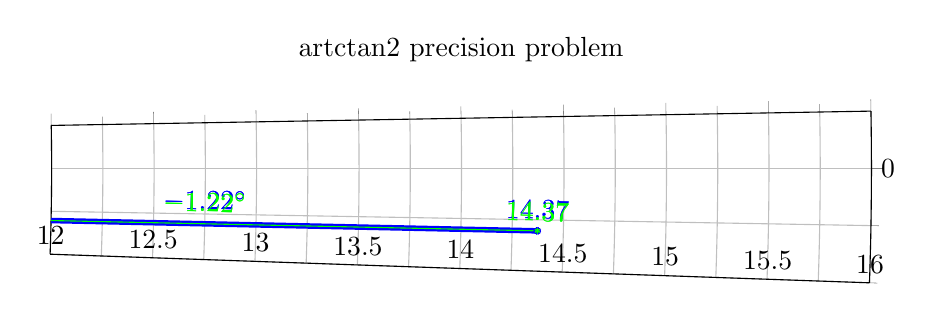
\begin{tikzpicture}
\begin{polaraxis}[
    visualization depends on=x \as \pgfplotspointx,
    nodes near coords,
    every node near coord/.style={
        %font=\small,
        rotate=\pgfplotspointx,
        append after command={
            node [
                anchor=south,
                %font=\small,
                rotate=\pgfplotspointx,
                shift={(axis direction cs:0,(12.75-\pgfplotspointmeta))}
            ] {$\pgfmathprintnumber{\pgfplotspointx}^\circ$}
        }
    },
width=7\textwidth,
xmin=-2,xmax=1, ymin=12, ymax=16,
title=artctan2 precision problem,
grid=both,
minor x tick num={4}, 
minor y tick num={1},
]
\addplot+[polar comb, data cs=cart, mark size=1, line width=2, mark=asterisk, color=blue, solid] table {
14.370195   -0.304948
14.370195   -0.304948

}; 
\addplot+[polar comb, mark size=1, mark=asterisk, color=green, solid] table {-1.215683667   14.37343027
-1.215683667    14.37343027
}; 
\end{polaraxis}
\end{tikzpicture}


\end{document}
